

In this paper we present Hypersliceplorer, an algorithm for generating 2D
slices of multi-dimensional shapes defined by a simplical mesh.  Often, slices
are generated by using a parametric form and then constraining parameters to
view the slice. In our case, we developed an algorithm to slice a simplical
mesh of any number of dimensions with a two-dimensional slice.  In order to get
a global appreciation of the multi-dimensional object, we show multiple slices
by sampling a number of different slicing points and projecting the slices into
a single view per dimension pair. These slices are shown in an interactive
viewer which can switch between a global view (all slices) and a local view
(single slice). We show how this method can be used to study regular polytopes,
differences between spaces of polynomials, and multi-objective optimization
surfaces. 

\begin{figure}
  \centering
  \begin{subfigure}[b]{0.45\linewidth}
    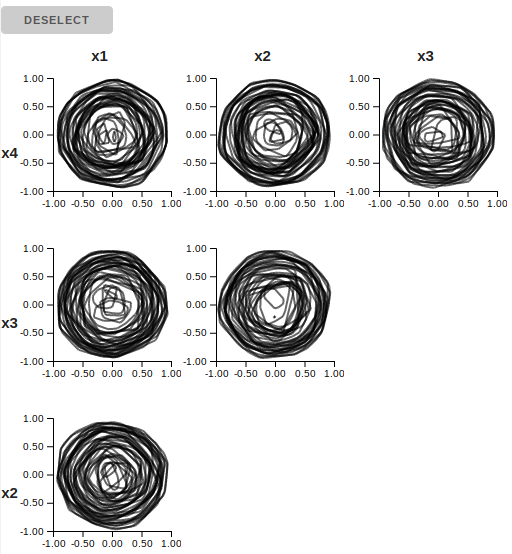
\includegraphics[width=\textwidth]{hsp_interface-global.png}
    \caption{Global view}
    \label{fig:interface:global} 
  \end{subfigure} 
  ~
  \begin{subfigure}[b]{0.45\linewidth}
    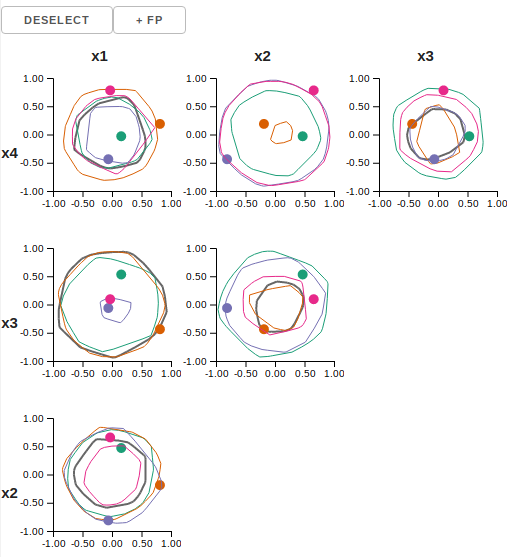
\includegraphics[width=\textwidth]{hsp_interface-local.png}
    \caption{Local view}
    \label{fig:interface:local} 
  \end{subfigure}
  \caption[The interface for browsing slices created by the Hypersliceplorer algorithm.]{%
    The interface for browsing slices created by the Hypersliceplorer algorithm.
    We show a plot for each pair of dimensions laid out in the same way as
    HyperSlice~\cite{Wijk:1993}.
    The interface has two modes: global and local view.
    The global view (\subref{fig:interface:global}) 
    shows the results of sampling over a number of focus points. The views
    are linked through highlighting a slice. The local view 
    (\subref{fig:interface:local}) shows a single selected slice and then
    the user can add additional slices by clicking the ``+ fp'' button.
  }
  \label{fig:interface}
\end{figure}

The visual analysis of multiple dimensions is one of the central themes of
visualization research. In principle there are two conceptual types of problems
that amount to two different mental models. (1) Often, the data set is considered to be truly discrete 
and projection methods, such as 
scatterplots and dimensionality reduction techniques, are used for its analysis.
Typical examples include business applications, in which one is analyzing
customer data.
The focus of
this paper is different in that (2) we are focusing on continuous multi-dimensional data spaces. For computational purposes, the data set is then merely a
set of points sampled from a continuous phenomenon of study. This is
rather common in simulation and engineering applications or for the study of
continuous algorithmic parameters in modeling environments, including machine
learning applications~\cite{Sedlmair:2014}. Of course, for such scenarios, projection based
visualization might be of help as well. However, they do not respect the mental
model of the object of study~\cite{Tory:2004}.

To comprehend these continuous data spaces, we extend the
HyperSlice~\cite{Wijk:1993} method, which presents a number of slices through
data space, all connected through one point in data space called the focus
point. Slicing has a number of advantages including undistorted views of the
space and the preservation of distances. The disadvantage is that only one
focus point can be shown at a time. Vastly different views of the object may be
seen depending on the location of the focus point. 
It is difficult to keep track of ones location while navigating multiple
dimensions.

In Sliceplorer~\cite{Torsney-Weir:2017a}, Torsney-Weir et al. suggest to
present 1D slices instead of 2D slices in such cases. While a 1D slice carries
less information than a 2D slice, they could now present a global view of the
multidimensional object by over-plotting many 1D slices. This advantage was
worth the loss of 2D information. In this paper, we take the idea of more global overviews and revisit 2D 
slices for closed multi-dimensional objects, whose overall multi-dimensional shape is
of great importance. This has been motivated by a number of real-world
application scenarios, from comprehension of multi-dimensional polytopes 
(generalization of polygons to multiple dimensions) by 
geometers, to applications in computational science, to
multi-dimensional Pareto-front analysis. By showing only slices of the outlines of these
polytopes we can again create global views of these data sets through
over-plotting of many focus points.

We address the issue of selecting a focus point by sampling a number of focus
points and producing projections of 2D slices (\autoref{fig:interface}). This
\emph{global view} gives the user an overview of the shape of the object
without having to navigate manually. Since we are viewing just
the outer hull of the object, we can draw these as a projection of a set of 2D
slices.  We use linked highlighting to show all slices for a particular focus
point.  In addition, the user can click on a particular slice and switch to the
\emph{local view}. The local view begins by showing the particular slice the
user clicked on. The user can add additional focus points and select particular
slices for comparison. This interaction models Shneiderman's mantra: ``overview
first, filter and zoom, details on demand''~\cite{Shneiderman:1996}.

Our major contribution is an
algorithm called Hypersliceplorer for computing the intersection of a 2D slice with a simplical
mesh in any dimension (see \autoref{sec:algorithm} and \autoref{fig:slicing}). The issue is that a 2D plane does not have a
well-defined normal in spaces higher than three. Therefore, we cannot
use the typical point-normal form of a plane in order to compute the
intersection of the plane with the simplex. Instead, we treat the plane
as a point with two free parameters representing the plane. Then, we
show how this representation allows us to compute how a
multi-dimensional simplex intersects a 2D plane. This approach lets us compute
slices of a multi-dimensional object without a parametric form of the
surface. We also demonstrate the results of this algorithm with an interactive
interface we developed.

We evaluate our algorithm and interface in two ways representing their recommended
evaluation methods according to the nested
model~\cite{Munzner:2009}. For the overall technique and
interactive viewer, we demonstrate the effectiveness of our technique by
presenting three case studies. For the underlying algorithm we present an
analysis of the running time. 

